
\section{Introduction}

\subsection{Micromouse competition}

According to the general description of the micromouse competition, "in this contest the contestant, or team of contestants, must design and build an autonomous robotic ”mouse” capable of traversing a maze of standard dimensions from a specified corner to its center in the shortest time." \cite{MicromouseRules}.\\
General example of a competition setup can be seen on the Fig.~\ref{fig:micromouse} 
\begin{figure}[htb]
    \centering
    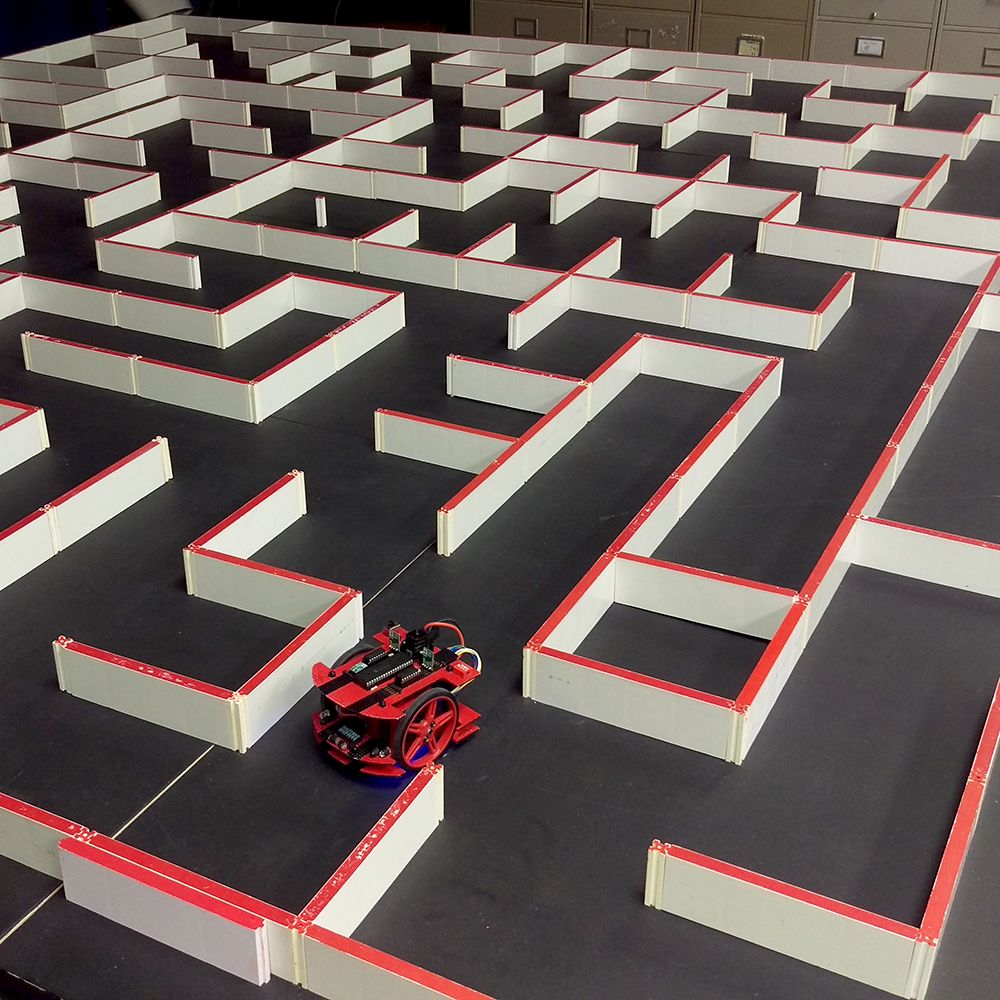
\includegraphics[width=0.6\textwidth]{figures/micromouse-maze.jpg}
    \caption{Micromouse competition photo: labyrinth and robot example \cite{MicromousePhotoLink}}
    \label{fig:micromouse}
\end{figure}

\subsection{Aims and Objectives}

    Short summary of the general competition rules is as following \cite{MicromouseRules}:

\begin{itemize}
    \item Self-Containment: A Micromouse shall be self-contained (no remote controls).
    \item Method of Movement: A Micromouse shall not jump over, fly over, climb, scratch,cut, burn, mark, damage, or destroy the walls of the maze.
    \item Maze Dimensions: The maze is composed of 18cm x 18cm unit squares arranged as 16 x 16 units. The walls of the units of the maze are 5 cm high and 1.2 cm thick 
    \item Multiple Paths: Multiple paths to the destination square are allowed and are to be expected. The destination square will be positioned so that a wall-hugging mouse will NOT be able to find it.
\end{itemize}
    
 In the case of our project, the aforementioned rules were used in a slightly modified way. The labyrinth is reduced in size to 8x8 units in order to fit better to the project conditions. The micromouse competition consists of 2 runs: in the first run, the robot is going through the maze and, according to arbitrary chosen algorithm, constructs the maze map; in the second run the mouse should reach the center of the maze (found in the first run) as quickly as possible, according to the composed map of the labyrinth. \\
 The main goal of the project was set to:  "get as close to the realization of the procedure described above as possible".
 The ways and approaches that were chosen to reach this goal are named and described properly in the next section.
 
 \subsection{Tools}
 
The list of tools used throughout the whole length of the project:
\begin{itemize}
    \item Microchip MPLABX - an IDE, used to set-up, configure and program a microcontroller. Used together with XC16 compiler from Microchip.
    \item MathWorks MATLAB \textcolor{red}{(did any of us except for Alex actually use it?)}
    \item Autodesk Eagle - PCB design software, used to create schematic diagrams, organize the component placement and route the PCB.
    \item Autodesk Fusion 360 -  CAD/CAM design software, used to build in 3D all parts of the casing for the robot.
\end{itemize}

